\section{Algorithims}
\label{sec:Algorithims}

This section describes two different algorhtims... These algorithims are similar to those described in...
\begin{figure}[H]
% Three counters
\newcounter{x}
\newcounter{y}
\newcounter{z}

% The angles of x,y,z-axes
\newcommand\xaxis{210}
\newcommand\yaxis{-30}
\newcommand\zaxis{90}


% The top side of a cube
\newcommand\topside[3]{
	\fill[fill=yellow, draw=black,shift={(\xaxis:#1)},shift={(\yaxis:#2)},
	shift={(\zaxis:#3)}] (0,0) -- (30:1) -- (0,1) --(150:1)--(0,0);
}

% The left side of a cube
\newcommand\leftside[3]{
	\fill[fill=red, draw=black,shift={(\xaxis:#1)},shift={(\yaxis:#2)},
	shift={(\zaxis:#3)}] (0,0) -- (0,-1) -- (210:1) --(150:1)--(0,0);
}

% The right side of a cube
\newcommand\rightside[3]{
	\fill[fill=blue, draw=black,shift={(\xaxis:#1)},shift={(\yaxis:#2)},
	shift={(\zaxis:#3)}] (0,0) -- (30:1) -- (-30:1) --(0,-1)--(0,0);
}

% The cube 
\newcommand\cube[3]{
	\topside{#1}{#2}{#3} \leftside{#1}{#2}{#3} \rightside{#1}{#2}{#3}
}

% Definition of \planepartition
% To draw the following plane partition, just write \planepartition{ {a, b, c}, {d,e} }.
%  a b c
%  d e
\newcommand\planepartition[1]{
	\setcounter{x}{-1}
	\foreach \a in {#1} {
		\addtocounter{x}{1}
		\setcounter{y}{-1}
		\foreach \b in \a {
			\addtocounter{y}{1}
			\setcounter{z}{-1}
			\foreach \c in {0,...,\b} {
				\addtocounter{z}{1}
				\ifthenelse{\c=0}{\setcounter{z}{-1},\addtocounter{y}{0}}{
					\cube{\value{x}}{\value{y}}{\value{z}}}
			}
		}
	}
}

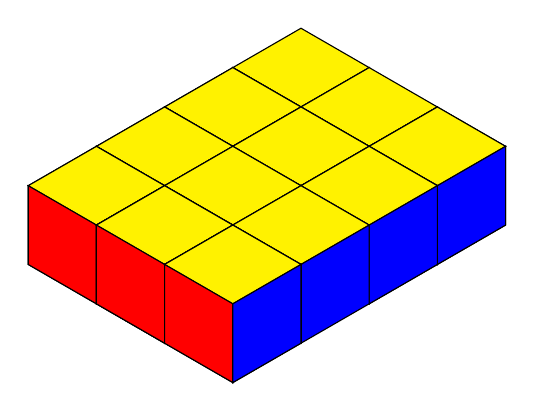
\begin{tikzpicture}
	\planepartition{{0,0,1},{1,1,1},{1,0,0},{1,2,1}}
\end{tikzpicture}


\caption{Mblocks with arrows}
\label{fig:CubeDiagram}
\end{figure}
	
\begin{algorithm}[htbp]
\hrulefill
\caption{Crystalization Algorithim}
\label{alg1}
\hrulefill
\begin{algorithmic}
\REQUIRE $n \geq 0$
\ENSURE $y = x^n$ 
\STATE $y \leftarrow 1$
\STATE $X \leftarrow x$
\STATE $N \leftarrow n$
 \WHILE{$N \neq 0$}
 \IF{$N$ is even}
\STATE $X \leftarrow X \times X$
\STATE $N \leftarrow N / 2$
\ELSE[$N$ is odd]
 \STATE $y \leftarrow y \times X$
\STATE $N \leftarrow N - 1$
\ENDIF
\ENDWHILE
\end{algorithmic}
\hrulefill
\end{algorithm}